\documentclass{acm_proc_article-sp}

\usepackage[T1]{fontenc}
\usepackage{polyglossia}
\setdefaultlanguage{english}
\usepackage{csquotes}

\usepackage{fontspec}
\usepackage{xltxtra}
\usepackage{libertine}

\usepackage[usenames, dvipsnames]{xcolor}
\graphicspath{{./img/}}

\usepackage[backend=biber, style=alphabetic]{biblatex}
\bibliography{literatur.bib}

\usepackage{subcaption}

\usepackage[%
unicode=true,%
colorlinks=true,%
linkcolor=black,%
urlcolor=MidnightBlue,%
citecolor=black,%
filecolor=black%
]
{hyperref}


\newcommand{\todo}[1]{\textcolor{Red}{#1}}
\newcommand{\sebastian}[1]{\textcolor{Green}{#1}}
\newcommand{\stefan}[1]{\textcolor{BurntOrange}{#1}}

\begin{document}

\title{
Interactive Simulation WS 15/16\\ %
Project Proposal
}
\subtitle{EYES - Exchange Your Vision Simulator}
\numberofauthors{2}
\author{
% 1st. author
\alignauthor
Sebastian Lemp\\
%       \affaddr{Street, House}\\
%       \affaddr{PLZ City}\\
%       \affaddr{Country}\\
%       \email{sebastian.lemp@student.uni-augsburg.de}
% 2nd. author
\alignauthor
Stefan Büttner\\
%       \affaddr{Street, House}\\
%       \affaddr{PLZ City}\\
%       \affaddr{Country}\\
%       \email{stefan.buettner@student.uni-augsburg.de}
}
%\additionalauthors{Additional Authors}

% The date is actually not used in the acm template
\date{University of Augsburg, \today}

% Not neede for our purposes
%\terms{Terms}
%\keywords{Keyword 1, Keyword 2}
%% A category with the (minimum) three required fields
%\category{H.4}{Information Systems Applications}{Miscellaneous}
%%A category including the fourth, optional field follows...
%\category{D.2.8}{Software Engineering}{Metrics}[complexity measures, performance measures]

%% For the ACM ToG format
%\acmformat{ACMFormat}
%\acmVolume{Vol.}
%\acmNumber{Nr.}
%\acmYear{YYYY}
%\acmMonth{MM}
%\acmArticleNum{XXX}
%\doi{DOI}


\maketitle
%\begin{abstract}
%\end{abstract}

% Disease list:
% -------------------------------------------------------------------------------
% (Stefan)     11 Disorders of sclera, cornea, iris and ciliary body
% (Sebastian)   1 Cataract (Grauer Star)
% (Stefan)      2 Retinal detachment and breaks
% (Sebastian)  14 Other retinal disorders
% (Stefan)      1 Glaucoma (Grüner Star)
% (Stefan)      2 Disorders of optic nerve and visual pathways
% (Sebastian)  10 Disorders of ocular muscles, binocular movement, accommodation and refraction
% (Stefan)      6 Visual disturbances and blindness
%              47

%
% Possible References:
% http://www.svi.cps.utexas.edu/EI466209.pdf

% http://www.icdvrat.org/2008/papers/ICDVRAT2008_S04_N06_Banks_McCrindle.pdf
%
% claim they have an real-time app for Android and iOS:
% http://www.brailleinstitute.org/sight-loss-blog/398-leading-eye-diseases.html 
%
% OpenGL real-time simulation
% http://percept.eecs.yorku.ca/papers/p127-vinnikov.pdf
% 

\section{Introduction/Motivation}
\begin{itemize}
  \item Give people the opportunity to experience different symptoms of eye
      disease, to know what they are and how to fight them for example
      nightblindness can caused by a wrong diet
      ⇒ so help people to eat the right food.
  \item Supposedly there is already a real-time simulator for eye diseases for
      Android, although we were not able to find it on Google Play Store for
      our phones \cite{braille}.
\end{itemize}

\section{Concept}

\begin{itemize}
  \item Fulfill everyday tasks with impaired vision
  \item Possible boni: 
  \begin{itemize}
    \item Get rid of disease by performing the right actions
    e.g. take medication on the way or make a doctors appointment...
    \item Preventive measures during the task to not get disease in next lvl
  \end{itemize}
  \item Target platform: Android \& Google Cardboard to address many people
\end{itemize}

\subsection{User Experience}

User should be able to experience different types of eye diseases, including
their early as well as the severe stages, in order to understand when to consult
a doctor and why. Hopefully this gives people better judgement on when to visit
a doctor as well as the courage to do so, if they experience the symptoms of
a particular disease.

\section{Project Requirements}

\begin{figure}
    \centering
    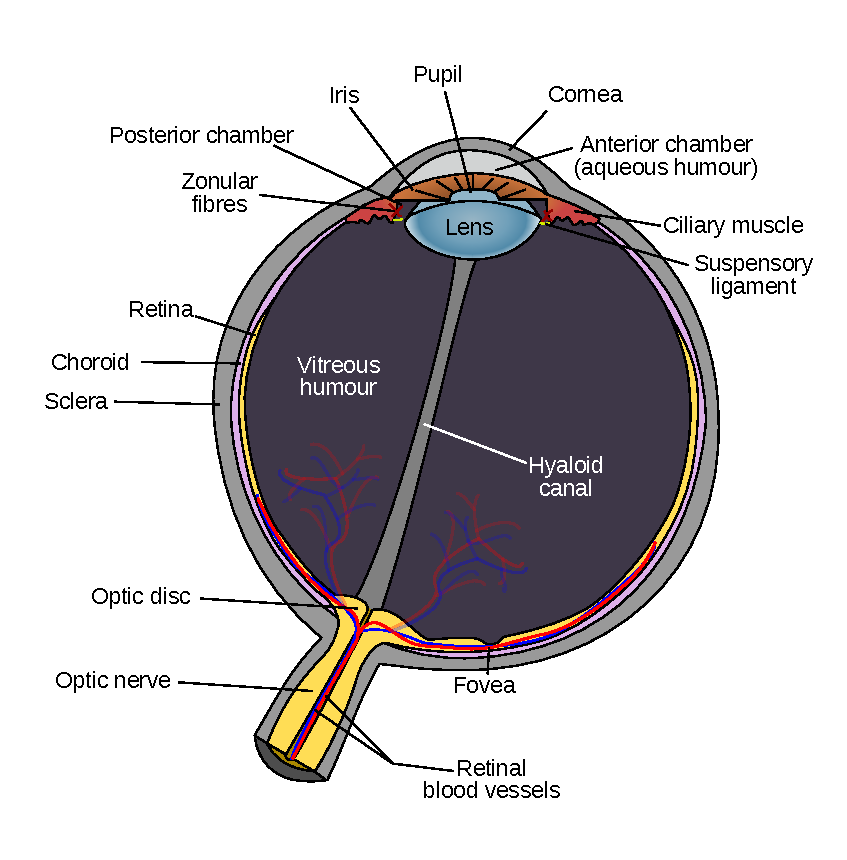
\includegraphics[width=\columnwidth]{human_eye_scheme.pdf}
    \caption{Scheme of the human eye.}
    \label{humaneye}
\end{figure}

\begin{description}
    \item[Glaucoma]
    \item[Cataracts]
        Blurred vision especially in the center region.

    \item[Diabetic Retinopathy]
        Black spots in the view

    \item[Color blindness]
        Some colours appear undistinguishable.

    \item[Achromatopsia]
        (Almost) No color sensitivity at all.

    \item[Myopia/Hyperopia]
        Commonly known as nearsightness and farsightness respectively.

    \item[Kreatoconus]
        Cornea shape converges to cone \\
        Multiple ghost images! (chaotic pattern),
        blurry vision, visual acuity at all distances, poor night vision
        photophobia, eye strain \\
        No to little pain \\
        Differently strong in both eyes

    \item[Nyctalopia/Hermalopia]
        High difficulty to see in relatively low and bright light respectively.

    \item[Retinal detachment/Posterior viterous detachment]
        Flashes of light, very brief in the extreme peripheral region.\\
        Sudden increase in the amount of floaters. \\
        Slight feeling of heaviness in the eye.

\end{description}

\section{Timeline}

\printbibliography

\balancecolumns

\end{document}
